%%%%%%%%%%%%%%%%%%%%%%%%%%%%%%%%%%%%%%%%%
% fphw Assignment
% LaTeX Template
% Version 1.0 (27/04/2019)
%
% This template originates from:
% https://www.LaTeXTemplates.com
%
% Authors:
% Class by Felipe Portales-Oliva (f.portales.oliva@gmail.com) with template 
% content and modifications by Vel (vel@LaTeXTemplates.com)
%
% Template (this file) License:
% CC BY-NC-SA 3.0 (http://creativecommons.org/licenses/by-nc-sa/3.0/)
%
%%%%%%%%%%%%%%%%%%%%%%%%%%%%%%%%%%%%%%%%%

%----------------------------------------------------------------------------------------
%	PACKAGES AND OTHER DOCUMENT CONFIGURATIONS
%----------------------------------------------------------------------------------------

\documentclass[
  french,
  twocolumn,
	9pt, % Default font size, values between 10pt-12pt are allowed
	%letterpaper, % Uncomment for US letter paper size
	%spanish, % Uncomment for Spanish
]{fphw}

\usepackage[fontsize=9.0]{scrextend} % Use this to force the fontsize
 % \usepackage{fancyhdr}
% Template-specific packages
\usepackage{babel}
\usepackage[utf8]{inputenc} % Required for inputting international characters
\usepackage{DejaVuSerifCondensed} 
\usepackage[T1]{fontenc} % Output font encoding for international characters
% \usepackage{mathpazo} % Use the Palatino font
% \usepackage{tgschola} % Use the Palatino font
% \usepackage{Alegreya}
% \renewcommand*\oldstylenums[1]{{\AlegreyaOsF #1}}
% \usepackage{iwona} % Use the Iwona font

\usepackage{fancyvrb}
\usepackage{fvextra}
\newcommand\userinput[1]{\textbf{#1}}
\newcommand\arguments[1]{\textit{#1}}

\usepackage{amsmath}
\usepackage{mathtools}
\usepackage{xfrac} 

\usepackage{graphicx} % Required for including images
\usepackage[textfont=it]{caption}  %% To manage long captions in images
\usepackage{subcaption}
\captionsetup{justification=centering}

\usepackage{float}
\graphicspath{ {./img/} }

\usepackage{booktabs} % Required for better horizontal rules in tables

\usepackage{listings} % Required for insertion of code

\usepackage{array} % Required for spacing in tabular environment

\usepackage{enumerate} % To modify the enumerate environment

\usepackage{amssymb}
\usepackage{enumitem}	%% % To modify the itemize bullet character

\usepackage{xcolor}
\usepackage{listings}
\colorlet{mygray}{black!30}
\colorlet{mygreen}{green!60!blue}
\colorlet{mymauve}{red!60!blue}
\lstset{
  backgroundcolor=\color{gray!10},  
  basicstyle=\ttfamily,
  columns=fullflexible,
  breakatwhitespace=false,      
  breaklines=true,                
  captionpos=b,                    
  commentstyle=\color{mygreen}, 
  extendedchars=true,              
  frame=single,                   
  keepspaces=true,             
  keywordstyle=\color{blue},      
  language=c++,                 
  numbers=none,                
  numbersep=5pt,                   
  numberstyle=\tiny\color{blue}, 
  rulecolor=\color{mygray},        
  showspaces=false,               
  showtabs=false,                 
  stepnumber=5,                  
  stringstyle=\color{mymauve},    
  tabsize=3,                      
  title=\lstname                
}

\usepackage[linkcolor=blue,colorlinks=true]{hyperref}
\usepackage{cleveref}
\usepackage{siunitx}
\newcommand{\bvec}[1]{\bm{#1}}    %% For vector notation
\newcommand{\myvec}[3]{\begin{pmatrix} #1  \\ #2 \\ #3 \end{pmatrix}}   %% vecteur 3d
\newcommand{\mymat}[9]{\begin{pmatrix} #1 & #2 & #3 \\ #4 & #5 & #6 \\ #7 & #8 &#9 \end{pmatrix}}  %% Matrice 3*3

\renewcommand{\vector}[4]{\begin{pmatrix} #1  \\ #2 \\ #3 \\ #4 \end{pmatrix}}   %% vecteur 3d
% \newcommand{\mymatrix}[16]{\begin{pmatrix} #1 & #2 & #3 & #4 \\ #4 & #6 & #7 & #8 \\ #9 & #10 & #11 & #12 \\ #13 & #14 & #15 & #16 \end{pmatrix}}  %% Matrice 3*3

\newcommand{\hquad}{\hspace{0.5em}} %% Bew command for half quad
% \setlength\parindent{0pt}	%% To remove all indentations

% \setlength{\parskip}{1em}%
% \setlength\parindent{0pt}

%----------------------------------------------------------------------------------------
%	ASSIGNMENT INFORMATION
%----------------------------------------------------------------------------------------

\title{Projet\\Aide aux librairies} % Assignment title

\author{Roussel Desmond Nzoyem} % Student name

\date{\today} % Due date

\institute{Université de Strasbourg \\ UFR de Mathématiques et Informatique} % Institute or school name

\class{Réseaux} % Course or class name

\professor{Pr. Pierre David} % Professor or teacher in charge of the assignment

%----------------------------------------------------------------------------------------

\begin{document}

% \maketitle % Output the assignment title, created automatically using the information in the custom commands above

%----------------------------------------------------------------------------------------
%	ASSIGNMENT CONTENT - SECTION 1
%----------------------------------------------------------------------------------------

\renewcommand{\abstractname}{Introduction}
\twocolumn[
  \begin{@twocolumnfalse}
    \maketitle
    \begin{abstract}
      \normalsize
      Nous proposons une implémentation d'un système permettant de collecter les demandes des clients et de les orienter vers des librairies, chez qui les clients pourront commander et chercher des livres en mode "click and collect". Notre implémentation repose sur le langage C et son API des sockets, suffisants pour faire fonctionner les différentes options traitées dans ce rapport.
    \end{abstract}
    \vspace*{0.5cm}
  \end{@twocolumnfalse}
]

\title{Aide aux librairies} %% Redefinition du titre pour les entetes de pages

\section{Description des protocoles}

Les différents éléments du système sont: les \textbf{librairies}, le serveur \textbf{Nil}, et les \textbf{clients}. Ces trois éléments communiquent entre eux à travers des protocoles bien spécifiques.


\subsection{Protocole Nil - Clients}

Le client transmet une demande au serveur Nil pour connaitre la disponibilité des certains livres. Nil répond avec une agrégation des différentes réponses des librairies qu'il a interrogé. Ces deux parties communiquent à travers le protocole TCP. Les segments échangés suivent la convention indiquée à la \cref{fig:nil-client}.
\begin{figure}[H]
	\centering
	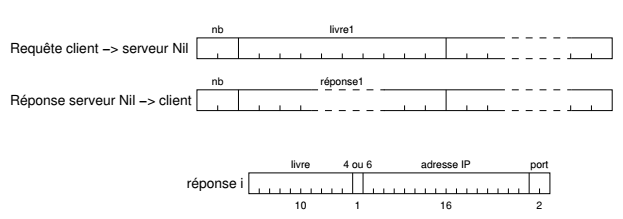
\includegraphics[width=0.4\textwidth]{nil-client.png}
	\caption{Protocole entre le serveur Nil et les clients.}
	\label{fig:nil-client}
\end{figure}

\subsection{Protocole Nil - Librairies}

Le serveur Nil retransmet la demande du client aux différentes librairies ; chaque librairie répond avec les livres qui sont disponibles. Ici, on utilise le protocole UDP afin d'imposer un délai au serveur pour répondre aux requêtes des clients. Les datagrammes échangés suivent la convention indiquées à la \cref{fig:nil-lib}.
\begin{figure}[H]
	\centering
	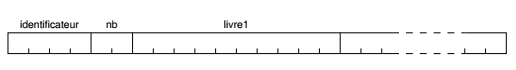
\includegraphics[width=0.4\textwidth]{nil-lib.png}
	\caption{Protocole entre le serveur Nil et les librairies.}
	\label{fig:nil-lib}
\end{figure}


\subsection{Protocole Librairie - Client}

Le client commande un livre auprès de la librairie ; la librairie confirme ou infirme la commande. Ici, on utilise le protocole TCP. Les segments échangés suivent la convention indiquée à la \cref{fig:lib-client}.
\begin{figure}[H]
	\centering
	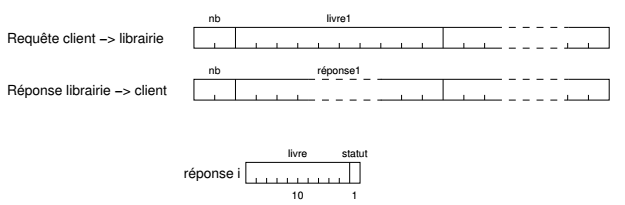
\includegraphics[width=0.4\textwidth]{lib-client.png}
	\caption{Protocole entre les librairies et les clients.}
	\label{fig:lib-client}
\end{figure}


\section{Implémentation}

Nous avons suivi une approche \textbf{agile} pour construire le programme. Les fonctionnalités les plus faciles ont été implémentées en premier, avant de passer aux plus complexes. L'ordre suivi fut le suivant :
\begin{enumerate}
  \item "envoi de requête" du client vers la librairie 
  \item "réception de requête" venant du client par la librairie
\end{enumerate}
$\Longrightarrow$ On possède la \textbf{version 1} du programme

\begin{enumerate}
  \setcounter{enumi}{2}
  \item "envoi de réponse" par la librairie au client
  \item "réception de réponse" venant de la librairie par le client ; et affichage des résultats 
\end{enumerate}
$\Longrightarrow$ On possède la \textbf{version 2} 

\begin{enumerate}
  \setcounter{enumi}{4}
  \item Communication Nil $\longleftrightarrow $ librairies
  \item Communication Nil $\longleftrightarrow $ clients
\end{enumerate}
$\Longrightarrow$ On possède la \textbf{version 3} finale
\\

\noindent À la fin du codage, on obtient un programme effectuant les différentes tâches demandées. Les fonctions de bibliothèques $\verb|getaddrinfo|$, $\verb|bind|$, $\verb|listen|$, $\verb|connect|$, et $\verb|select|$ ont régulièrement été utilisées dans la construction de chacun des composants. En particulier, la fonction $\verb|getaddrinfo|$ a été utilisée pour "résoudre" les adresses IP, qu'elles soient en IPv6 ou en IPv4.


%----------------------------------------------------------------------
\subsection{Clients}

Il s'agit d'un client TCP classique qui communique avec un serveur, le serveur pouvant être Nil ou une librairie ; la commande à exécuter est la suivante :
\begin{Verbatim}[commandchars=\\\{\}]
$ \userinput{client} \arguments{serveur port livre1 livre2 ... livren}
\end{Verbatim}

\noindent Les étapes principales de son implémentation, contenues dans le fichier $\verb|client.c|$, sont les suivantes :

\begin{enumerate}
  \item Récupération de l'adresse IP du serveur à travers la fonction $\verb|getaddrinfo|$ (protocole IPv6 pouvant supporter IPv4)
  \item Création d'un socket pour se connecter au serveur (aucun $\verb|bind|$ n'est nécessaire) 
  \item Ouverture active de connexion vers le serveur à travers la fonction $\verb|connect|$
  \item Envoi de la demande au serveur à travers la fonction $\verb|write_to_server|$
  \item Création d'une boucle infinie pour attendre la réponse du serveur à travers la fonction $\verb|select|$
  \item Lecture du contenu du message à travers la fonction $\verb|read_from_server|$. C'est à ce niveau que la distinction entre un serveur de type "Librairie" ou un serveur de type "Nil" s'opère ; le client lit l'octet numéro 13 de la réponse:
  \begin{itemize}
    \item Si cet octet contient la valeur 0 ou 1 : alors la réponse provient d'une librairie
    \item Si cet octet contient la valeur 4 ou 6 : alors la réponse provient de Nil
    \item Sinon, ce segment TCP n'est pas valide
  \end{itemize}
\end{enumerate}


\subsection{Librairies}

Il s'agit d'un serveur fonctionnant à la fois en TCP et en UDP. La commande à exécuter est la suivante :
\begin{Verbatim}[commandchars=\\\{\}]
$ \userinput{librairie} \arguments{port livre1 livre2 ... livren}
\end{Verbatim}
\textbf{Remarque}: \textit{L'adresse IP de la librairie n'est pas fournie à la création. Cette adresse correspond à l'adresse IP utilisée par l'interface (de la machine sur laquelle est lancée la librairie) pour communiquer avec le reste de l'internet}.
\\

\noindent Le fichier correspondant se nomme $\verb|librairie.c|$, et les étapes principales de l'implémentation sont les suivantes :
\begin{enumerate}
  \item Création du socket UDP pour la communication avec le serveur Nil
  \item Bind du socket au port défini pour cette librairie (donné en argument)
  \item Création du socket TCP pour la communication avec le client
  \item Bind du socket au même port que précédemment
  \item Mise en écoute sur le port TCP pour au plus $\verb|MAX_CLIENTS_NB|$ \footnote{Attention, cette directive de préprocesseur est définie différemment pour la librairie et pour le serveur Nil.} clients ; ceci à travers la fonction $\verb|listen|$.
  \item Création d'une boucle infinie pour attendre des connexions entrantes de Nil ou d'un client. Tout comme lors de l'implémentation du client, nous devons utiliser la fonction $\verb|select|$ à ce niveau.
  \item En cas d'un évènement de type "écriture" sur l'un des sockets :
  \begin{itemize}
    \item S'il s'agit du socket UDP : alors traiter la demande du serveur Nil
    \item S'il s'agit du socket TCP : alors faire une ouverture passive de connexion à travers la fonction $\verb|accept|$ ; ensuite traiter la commande du client (ne pas oublier de mettre à jour le stock de livres de la librairie)
  \end{itemize}
\end{enumerate}

\subsection{Nil}
\label{sec:subnil}

La pièce centrale du système fonctionne à la fois en tant que client UDP et serveur TCP. La commande à exécuter est la suivante :
\begin{Verbatim}[commandchars=\\\{\}]
$ \userinput{nil} \arguments{port délai librairie port librairie port...}
\end{Verbatim}
\textbf{Remarque}: \textit{Tout comme avec la librairie, l'adresse IP n'est pas fournie. Elle est déduite de la machine qui crée le serveur.}
\\

\noindent Le fichier correspondant se nomme $\verb|nil.c|$, et les étapes principales de son implémentation sont les suivantes :

\begin{enumerate}
	\item Créer un unique socket TCP pour communiquer avec tous les clients
  \item Bind du socket TCP au port défini pour le serveur
  \item Se mettre en écoute sur le port TCP
  \item Résoudre les adresses IP des différentes librairies
  \item Créer autant de sockets UDP qu'il y a de librairies $\verb|nb_libs|$. Un $\verb|bind|$ des sockets au port défini pour le serveur Nil n'est pas nécessaire.
  \item Créer une boucle infinie pour attendre des requêtes de clients, ou des réponses de librairies 
	\item En utilisant $\verb|select|$, écouter des événements de type "écriture" sur les $\verb|nb_libs+1|$ sockets surveillés, pendants au plus $\verb|délai|$ secondes :
	\begin{itemize}
		\item Si le $\verb|select|$ s'arrête à cause de l'arrivée d'un nouveau client : utiliser l'identifiant prévu pour le client, et retransmettre la requête du client vers toutes les librairies. Sachant qu'un meilleur identifiant sera probablement libéré, prendre le $\verb|next_id|$\footnote{Il s'agit de l'identifiant à utiliser pour le prochain client entrant} comme étant le plus grand identifiant utilisé jusqu'à présent plus 1.
		\item Si le $\verb|select|$ s'arrête à cause de la réponse d'une librairie : identifier le client concerné par la réponse, et mettre à jour son buffer de réponse. Si on constate que ce client a été concerné déjà autant de fois qu'il y a de librairies, alors on peut lui envoyer sa réponse ; ensuite il faut mettre à jour le $\verb|next_id|$ ; on prendra cet identifiant (devenu disponible) s'il est plus petit que le $\verb|next_id|$ actuel.
		\item Si le $\verb|select|$ s'achève par un "timeout" : alors tous les clients encore actifs ont attendu plus de $\verb|délai|$ secondes sans réponse. Il faut donc renvoyer les réponses correspondantes à chacun de ces clients ; ensuite mettre à jour $\verb|next_id|$ ; on prendra le plus petit des identifiants devenus disponibles. 
	\end{itemize}
\end{enumerate}


\section{Structures de données}

Les structures de données non triviales mises en \oe{}uvre sont les suivantes :

\begin{itemize}
  \item Les types $\verb|uint8_t, uint16_t, uint32_t, et uint64_t|$ pour respecter les limitations de chaque protocole, et avoir un code portable.
	\item Les pointeurs sur des $\verb|uint8_t|$ pour les buffers, qui vont constituer les segments TCP ou les datagrammes UDP échangés.
	\item Pour le serveur Nil :
	\begin{itemize}
    \item Des tableaux statiques pour sauvegarder les états des librairies (adresses IP, descripteurs de sockets, etc.), dont le nombre est bien connu à l'avance.
    \item Des tableaux alloués dynamiquement pour sauvegarder les états des clients (activité, buffer de réponse, taille du buffer de réponse, etc.). Sachant qu'on peut avoir jusqu'à $2^{32} - 1$ clients simultanément, on décide d'allouer initialement de l'espace pour n'en traiter que $32$. En cas de nécessité, on étendra cet espace.
  \end{itemize}

\end{itemize}


\section{Test visuel}
\label{sec:test}

Nous avons effectué une simulation sur un réseau local $\verb|192.168.188.0/24|$ spécialement créé à cet effet \footnote{La nécessité d'utiliser un réseau local vient du besoin d'éviter les pare-feux et les mots de passe nécessaires pour se connecter en SSH par exemple.}. La machine principale (celle sur laquelle nous lançons le serveur Nil et le client) a pour adresse IP $\verb|192.168.188.152/24|$. Les différents éléments de la simulation sont les suivants : 
\begin{itemize}
  \item La librairie \#1 est créée sur la machine principale, et contient les livres B, C, A, et Zoro : \begin{Verbatim}[commandchars=\\\{\}, breaklines=true, breakanywhere=true] 
    $ \userinput{librairie} \arguments{9001 B C A Zoro}
    \end{Verbatim} 
  \item La librairie \#2 est créée sur la machine principale, et contient les livres Azimov et Dune : \begin{Verbatim}[commandchars=\\\{\}, breaklines=true, breakanywhere=true]
    $ \userinput{librairie} \arguments{9002 Azimov Dune}
    \end{Verbatim} 
  \item La librairie \#3 est créée sur une machine du réseau local $\verb|192.168.188.141/24|$, et contient les livres Zoro et A : \begin{Verbatim}[commandchars=\\\{\}, breaklines=true, breakanywhere=true]
    $ \userinput{librairie} \arguments{9003 Zoro A}
    \end{Verbatim} 
  \item La librairie \#4 est créé sur la machine $\verb|turing.u-strasbg.fr|$ et ne contient aucun livre : \begin{Verbatim}[commandchars=\\\{\}, breaklines=true, breakanywhere=true]
    $ \userinput{librairie} \arguments{9004}
    \end{Verbatim} 
  \item Le serveur Nil est créé sur la machine principale et interroge les 4 librairies : \begin{Verbatim}[commandchars=\\\{\}, breaklines=true, breakanywhere=true]
    $ \userinput{nil} \arguments{9000 5 127.0.0.1 9001 ::1 9002 192.168.188.141 9003 turing.u-strasbg.fr 9004}
    \end{Verbatim} 
  \item Le client est créé sur la machine principale et interroge le serveur Nil: \begin{Verbatim}[commandchars=\\\{\}, breaklines=true, breakanywhere=true]
    $ \userinput{client} \arguments{::1 9000 Dune Zoro Perl Taron A Azimov}
    \end{Verbatim} 
\end{itemize}


\begin{figure*}[h]
  \centering
  \begin{subfigure}{0.422\textwidth}
    \centering
    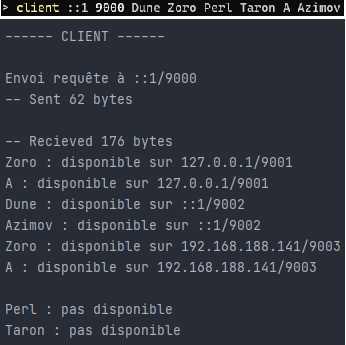
\includegraphics[width=\textwidth]{client.png}
    \caption{Client}
    \label{fig:client}
  \end{subfigure}
  \begin{subfigure}{.478\textwidth}
    \centering
    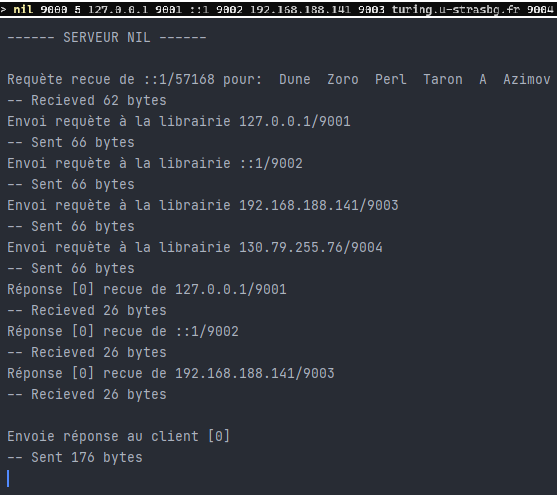
\includegraphics[width=\textwidth]{serveur_nil.png}
    \caption{Serveur Nil}
    \label{fig:nil}
  \end{subfigure}
  \begin{subfigure}{0.245\textwidth}
    \centering
    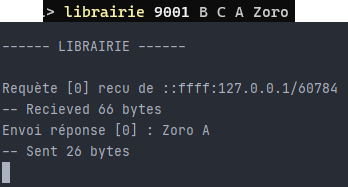
\includegraphics[width=\textwidth]{librarie1.png}
    \caption{Librairie 1}
    \label{fig:lib1}
  \end{subfigure}
  \begin{subfigure}{0.195\textwidth}
    \centering
    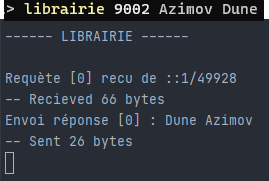
\includegraphics[width=\textwidth]{librarie2.png}
    \caption{Librairie 2}
    \label{fig:lib2}
  \end{subfigure}
  \begin{subfigure}{0.28\textwidth}
    \centering
    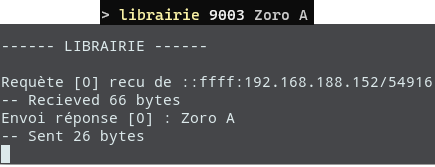
\includegraphics[width=\textwidth]{librarie3.png}
    \caption{Librairie 3}
    \label{fig:lib3}
  \end{subfigure}
  \begin{subfigure}{0.24\textwidth}
    \centering
    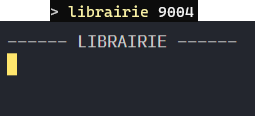
\includegraphics[width=\textwidth]{librarie4.png}
    \caption{Librairie 4}
    \label{fig:lib4}
  \end{subfigure}
  \caption{Affichage de chacune des parties lors de la simulation du fonctionnement du système. Les commandes exécutées par chacune des parties, reprises ici, sont détaillées à la \cref{sec:test}. Ces résulats indiquent que le client peut décider de faire, avec succès, une commande auprès des librairies 1, 2, ou 3. C'est cela qu'on observe à la \cref{fig:simu2}.}
  \label{fig:simu}
\end{figure*}



\begin{figure*}[h!]
  \centering
  \begin{subfigure}{0.35\textwidth}
    \centering
    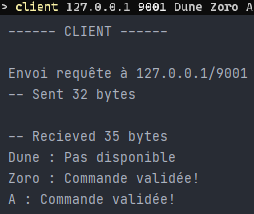
\includegraphics[width=\textwidth]{commandA.png}
    \caption{Client}
    \label{fig:com1}
  \end{subfigure}
  \begin{subfigure}{.45\textwidth}
    \centering
    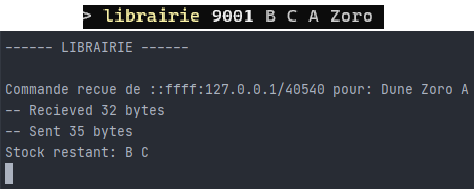
\includegraphics[width=\textwidth]{commandB.png}
    \caption{Librairie 1}
    \label{fig:com2}
  \end{subfigure}
  \caption{Simulation d'une commande de deux livres par un client auprès d'une librairie. Cette simulation complète celle observée à la \cref{fig:simu}, et permet d'observer le protocole Librairie - Client à l'\oe{}uvre. Notons que cette simulation n'a pas été faite immédiatement après la fin de la requête auprès de Nil. Sinon, on aurait observé un affichage continu du côté de la librairie, et le port attribué au client par l'OS aurait sans doute été le même.}
  \label{fig:simu2}
\end{figure*}


\noindent Les résultats obtenus sont présentés à la figure \cref{fig:simu}. On y observe plusieurs points qui font la force de ce programme :
\begin{itemize}
  \item Les système fonctionne correctement en IPv6 comme en IPv4. En réalité, il fonctionne en IPv6 et les adresses IPv4 sont convenablement converties en IPv6 (cf. \cref{fig:lib1,fig:lib3}).
  \item La librairie \#4 située sur $\verb|Turing|$ (d'adresse IP $\verb|130.79.255.76|$) n'est pas accessible à partir du réseau local créé (cf. \cref{fig:nil}), a moins d'établir une connexion SSH. Cela n'empêche pas le programme de fonctionner ; et une réponse est retournée au client après que le délai de $\verb|5|$ secondes s'est écoulé.
\end{itemize} 

\noindent Les atouts de notre implémentation du serveur $\verb|nil|$, qui ne sont pas directement observables depuis la \cref{fig:simu} sont : 
\begin{itemize}
  \item Le serveur ne nécessite pas de $\verb|fork|$, tout se passe dans le processus créé initialement ; ce qui facilite le débogage en cas de problème.
  \item Le serveur supporte jusqu'à $\verb|MAX_CLIENTS_NB|$ $\verb|= 4294967295|$ clients simultanément. Pour ce faire de manière efficace, on a recours à une attribution des identifiants de manière astucieuse (décrite à la \cref{sec:subnil}), qui permet d'économiser la mémoire RAM utilisée. Cela est d'autant plus important que le serveur Nil (tout comme les différentes librairies) peut tourner indéfiniment sans jamais s'arrêter.
\end{itemize}


\section{Limitations}

Les principales limitations du programme sont les suivantes :

\begin{itemize}
  \item \textbf{Plusieurs ports UDP} sont utilisés par le serveur pour communiquer avec les librairies (cf. \cref{fig:lib1,fig:lib2,fig:lib3}), ce qui peut être prohibitif si l'on a un grand nombre de librairies à interroger. Cette difficulté a été introduite par le fait que les adresses IP utilisées pour se connecter aux librairies peuvent varier (IPv4, IPv6, adresse IP secondaire) ; en plus, une adresse valide lors d'une première connexion peut ne plus être valide lors de la suivante. La résolution de ce problème nécessite un $\verb|bind|$ au port dédié au serveur Nil\footnote{En IPv6, une liaison (ou "bind") au port dédié a pu être établie ; cependant en IPv4, des difficultés ont été rencontrées.}. 
  \item Le \textbf{nombre de clients} qu'une librairie peut mettre dans sa file d'attente est raisonnablement limité à $\verb|MAX_CLIENTS_NB=65335|$. Autrement dit, si plus de $\verb|65335|$ clients essaient simultanément de commander  des ouvrages auprès de la même librairie, certaines commandes seront simplement ignorées.
  \item La \textbf{tolérance aux pannes} (qui consiste à émettre une nouvelle requête à destination d'une librairie si Nil n'a pas reçu de réponse après le délai imposé) n'a pas été implémentée. Le processus a cependant été initié. Pour le mener à terme, il faudrait utiliser le tableau $\verb|active_clients|$ qui indique l'activité de tous les clients :
  \begin{itemize}
    \item Si $\verb|active_clients[j] = 0|$, alors, de l'espace a été alloué pour recevoir le client $\verb|j|$, mais celui-ci n'existe pas encore; ou alors ce client à déjà entièrement été traité.
    \item Si $\verb|active_clients[j] = 1|$, alors le client $\verb|j|$ a attendu pendant $\verb|délai/2|$ secondes, mais n'a toujours pas reçu la totalité des $\verb|nb_libs|$ réponses qu'il a besoin. Il faut donc renvoyer une requête aux librairies concernées par le retard.
    \item Si $\verb|active_clients[j] = 2|$, alors le client $\verb|j|$ a attendu pendant $\verb|délai|$ secondes, mais n'a toujours pas reçu ses $\verb|nb_libs|$ réponses. Dans ce cas, il faut immédiatement renvoyer la réponse au client. 
  \end{itemize}
  On constate que pour résoudre ce dernier problème, il faut garder en mémoire non seulement la requête que chaque client a effectué auprès du serveur Nil, mais aussi quelles librairies n'ont pas répondu à la demande de Nil. 
\end{itemize}






\end{document}
